\documentclass[a4paper,11pt]{jsarticle}
%\usepackage{latexsym}
%\usepackage{epsfig}
\usepackage[dvipdfmx]{graphicx}
\usepackage{epsfig}
%\usepackage{graphicx}
\usepackage{amsmath}
\usepackage{amssymb}
\usepackage{theorem}
\usepackage{multicol}
\usepackage{mdwlist}
\usepackage{url}
\usepackage[colorlinks=true,urlcolor=cyan,linkcolor=blue,dvipdfmx]{hyperref}
\usepackage[dvipdfmx]{hyperref}
\usepackage{pxjahyper}
\usepackage{simplebnf}
\usepackage{mathtools}

\usepackage{subcaption}
\usepackage{listings}
\usepackage{float}
\usepackage{here}

\lstset{
  basicstyle=\ttfamily\small,
  numbers=left,
  numberstyle=\small,
  numbersep=8pt,
  frame=shadowbox
}

%\pagestyle{empty}

\title{{\bf 情報システム実験I\\コンパイラ}}
\author{伊澤侑祐}
\date{}

\begin{document}
\maketitle

\section{実験目的}
本実験では、コンパイラの実装を通してある程度複雑なソフトウェアの実装手法を体験します。
コンパイラは愚直に実装しようとすると大変ですが、これまで多くの実装手法が研究・開発されてきました。
具体的には、While 言語という、制御構造として繰り返し構造のみを持った言語のコンパイラを実装
し、その開発手法の一旦を垣間見ることがきます。

% 図~\ref{phase}にコンパイル処理の流れを示します。\framebox[1cm][l]{ }で囲まれた各フェーズ
% の具体的な処理については、\ref{text}節に示したテキスト「\textbf{コンパイラI}」と
% 「\textbf{コンパイラII}」を参照して下さい。

本実験の目的は以下の通りです。

\begin{enumerate}
\item Pscal 風の高級言語 (While言語) を仮想的なスタック機械の命令コードに翻訳する仕組みを学ぶ。
\item 仮想的なスタック機械の命令コードを経由してPython命令コードへ翻訳する仕組みを学ぶ。同
  時に、実際にPythonインタプリタでWhile言語コンパイラを動作させてみる。
\item スタック機械である Python インタプリタの仕組みの概観を理解する。
\item Visual Studio Code に慣れる。
\end{enumerate}

\section{テキスト}\label{text}
%下記のテキストを読んで,各自で課題をこなす.
%実習書には,実験の目的,言語の仕様,参考書へのポインタ,レポート内容など実験特有の情報を記述する.

以下の本(\textbf{Pascal}以外)をテキストとして、それぞれを1人1冊貸し出します。
必要なら各自の責任の元に、貸し出し帳に記入の上持ち帰っても構いません。
テキストの参照箇所を示す時、テキスト名を\textbf{コンパイラI}のように略して表記しています。
OCaml については、五十嵐淳教授 (京都大学) の「OCaml爆速入門」を「手を動かしながら」読んで
ください。最初の授業でも解説します。

\begin{description}
\item[OCaml爆速入門]
  「\href{https://www.fos.kuis.kyoto-u.ac.jp/~igarashi/class/pl/03-ocaml.html}{OCaml爆速
    入門}」、五十嵐淳、2019年
\item[コンパイラI] 「コンパイラ I 言語・技法・ツール」,A.V.エイホ他著,サイエンス社,1990年
\item[コンパイラII] 「コンパイラ II 言語・技法・ツール」,A.V.エイホ他著,サイエンス社,1990年
\item[Pascal] 「Pascal」,K.イェンゼン他著,培風館,1993年
\end{description}

\section{コンパイラ}
\label{sec:compiler}

コンパイラとは、ある言語で書かれたソースコードを読み込んで、コンピュータが実行できる機械語
に翻訳するプログラムです。多くの場合、高級言語と呼ばれるC言語やPascalなど人間が理解しやす
い言語で記述されたソースコードをCPU(中央演算処理装置)が実行できる命令コードに変換するプ
ログラムを指します。

具体的には、コンパイラはユーザによって書かれたプログラムから動作させたい機械 (CPUなどの計
算装置) が実行できるプログラムへ変換します。
コンパイラの入力言語は\textbf{ソース言語}、ソース言語で書かれたプログラムを\textbf{ソースプログラ
ム}と呼びます。一方、動作させたい機械のことを\textbf{ターゲット機械}、最終的に変換されるプ
ログラムを\textbf{ターゲットプログラム}などと呼びます。

図~\ref{fig:compilation_flow}は、一般的なコンパイラのコンパイルフローを表してい
ます。コンパイラはソースプログラムを一気にターゲットプログラムへ変換するのではなく、何段階
かのコード変換フェーズを経ることによって変換しています。

\begin{figure}[t]
  \centering
  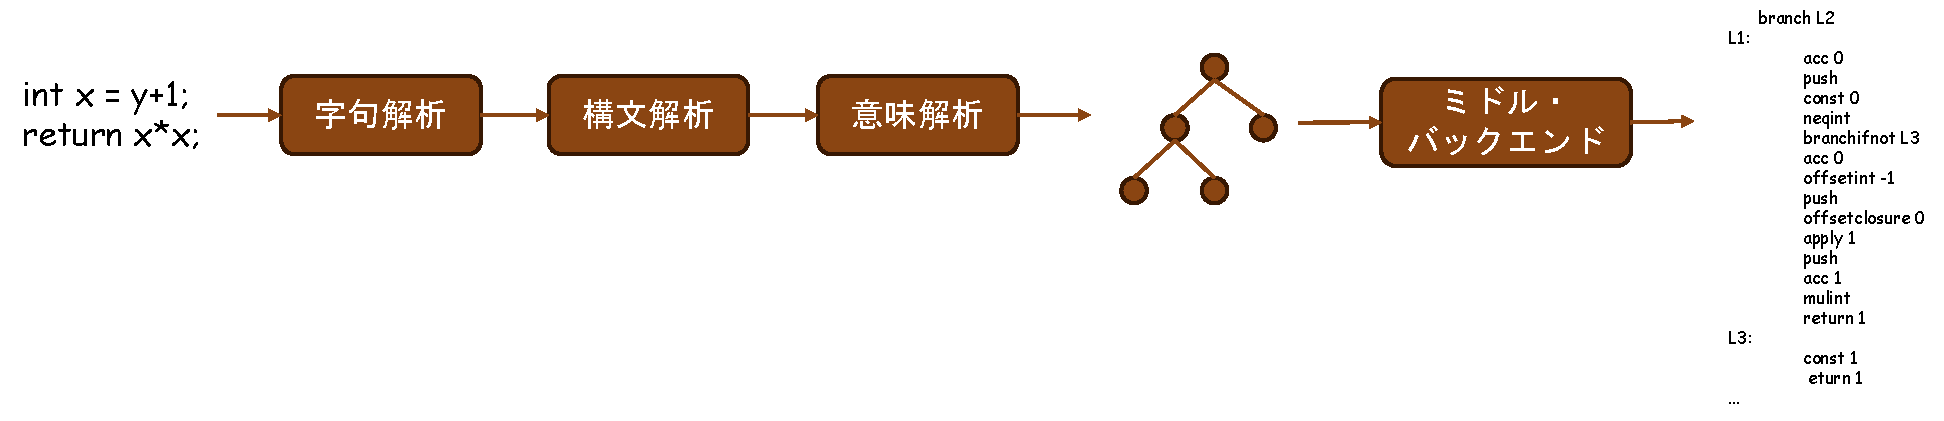
\includegraphics[width=\linewidth]{figs/compiler_structure_overview.pdf}
  \caption{一般的なコンパイラのコンパイルフロー図}
  \label{fig:compilation_flow}
\end{figure}

% 面白い例え: https://www.momoyama-usagi.com/entry/info-calc-sys11
次に、コンパイラのコンパイルフローの概要を説明します。コンパイラは、まず、ユーザが記述した
While 言語プログラム (ソースプログラム) を入力として受
けとります。次に、\textbf{字句解析器}がソースプログラムを\textbf{字句} (\textbf{トークン}、
\textbf{token}) へ分割し、字句の種類を識別する\textbf{字句解析 (Lexical Analysis)}を行い
ます。次に、\textbf{構文解析器}が字句の列を整理し文構造を把握する\textbf{構文解析 (Syntax
  Analysis)} を行い\textbf{構文木 (シンタックス・ツリー、syntax tree)} へ変換します。次に、
変換された構文木に意味的な誤りがないかチェックする
\textbf{意味解析 (Semantic Analysis)} を行います (本実験では意味解析の実装は時間の都合上ス
キップします)。意味解析が完了し誤りがないことが分かったら、構文木を\textbf{中間表現
  (Intermediate Representation)} へ変換します。中間表現を対象に、プログラムを高速に動かす
ため、未使用定義の削除や関数呼出の展開といった\textbf{最適化 (Optimization)} を行います。
最適化が終わったら、最後にターゲットプログラムを生成 (\textbf{コード生成、Code
  Generation}) します。各フェーズの詳しい説明は\textbf{コンパイラ}第2章あるいは第3章以降の該当ページを参照してください。

\section{While言語とWhile言語コンパイラ}
\label{sec:while_lang}

\subsection{While言語の仕様}
%テキストの909ページ付録に構文例がのっているので参考にする.

% ソースコードを記述する言語をソース(原始)言語と呼びます。
本実験では、図~\ref{spec}の仕様を持つ While 言語のコンパイラを実装します。仕様の中にある変数の意味は、直前の定義を参照してください。
この書き換え規則により、例えば代入文 ``\textsf{i := i + 1}'' が生成できます(図~\ref{生成例})。
また、図~\ref{sample}に$9$の階乗を計算するプログラムの例を示します。

\begin{figure}[H]
  \centering
  \begin{description}
\item[S] 文 (statements)
\item[a] 算術式 (arithmetic expressions, arith)
\item[x,y] 変数 (program variables)
\item[n] 数値 (number literals)
\item[P] 真偽値 (boolean variables)
\end{description}

\begin{bnf}
  $S$ : \textsf{文} ::= $x$ $\coloneq$ $a$
  | skip
  | $S_1$; $S_2$
  | if $P$ then $S_1$ else $S_2$
  | while $P$ begin $S$ end
  ;;

  $a$ : \textsf{算術式} ::= $x$
  | $n$
  | ( $a$ )
  | $a_1$ $op_a$ $a_2$
  ;;

  $op_a$ : \textsf{算術演算} ::= $+$ || $-$ || $\star$ || $/$
  ;;

  $P$ : \textsf{真偽値} ::= true
  | false
  | not $P$
  | $P_1$ $op_b$ $P_2$
  | $a_1$ $op_r$ $a_2$
  ;;

  $op_b$ : \textsf{真偽演算} ::= and || or
  ;;

  $op_r$ : \textbf{比較演算} ::= $<$ || $>$ || $\leq$ || $\geq$ || $==$
  ;;
\end{bnf}
  \caption{ソース言語の仕様}\label{spec}
\end{figure}

\begin{figure}[H]
  \begin{subfigure}[b]{.4\linewidth}
    \centering
    \textsf{\small
      \begin{tabular}{lcl}
        S    & $\rightarrow$ & x := a \\
             & $\rightarrow$ & i := a \\
             & $\rightarrow$ & i := a + a \\
             & $\rightarrow$ & i := x + a \\
             & $\rightarrow$ & i := i + a \\
             & $\rightarrow$ & i := i + n \\
             & $\rightarrow$ & i := i + 1
      \end{tabular}
    }
    \caption{文の生成例}\label{生成例}
  \end{subfigure}\hfill
  \begin{subfigure}[b]{.5\linewidth}
    \centering
    \begin{lstlisting}
      a := 1;
      i := 2;
      while i < 10 do
      begin
        a := a * 1;
        i := i + 1;
      end
    \end{lstlisting}
    \caption{プログラム例}\label{sample}
  \end{subfigure}
\end{figure}

\subsection{While言語コンパイラの構造}

本実験で実装する While 言語
(詳しい解説は第~\ref{sec:while_lang}節を参照) コンパイラのコンパ
イルフロー (コンパイルの段階を段階ごとに示したもの) です。

\begin{figure}[t]
  \centering
  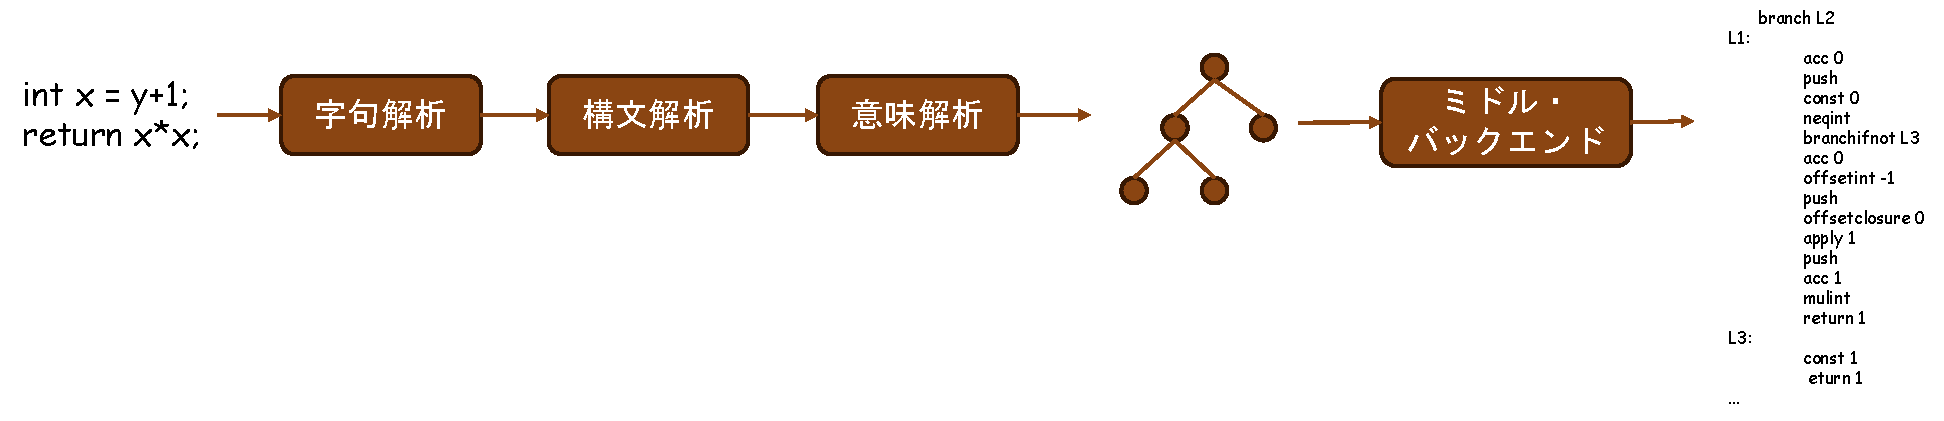
\includegraphics[width=\linewidth]{figs/compiler_structure_overview.pdf}
  \caption{本実験で実装するコンパイラのコンパイルフロー図}
  \label{fig:compilation_flow_while_lang}
\end{figure}


\section{仮想スタック機械の仕様}
本実験では中間表現としては仮想的なスタック機械 (仮想機械) の仮想命令を利用します。仮想機械
とは、Intel CPU や Ryzen CPU といった具体的な機械ではなく、それらを抽象化した機械のことで
す。VirtualBoxのような仮想環境ではなく、JavaやPythonなどの処理系を思い浮かべてください。そ
れらがいわゆる仮想機械を用いて実現されています。
仮想的なスタック機械の詳細は\textbf{コンパイラI}の2章2.8節を参
照して下さい。表~\ref{stackcommand}にスタック機械の命令セットを示します。なお、Pythonバイ
トコードへの変換のため、教科書にある命令セットを一部変更しています。

\begin{table}[H]
\caption{スタック機械の命令セット} \label{stackcommand}
\centering
\normalsize{
  \begin{tabular}{c|p{30zw}}
    \hline
    \texttt{push} $v$ & $v$をスタックに積む。\\
    \texttt{pop} & スタックの最上段の要素を取り去る。\\
    $+$ & 最上段とその下にある要素を取り出して加算し、結果をスタックに積む。\\
    $-$ & 最上段とその下にある要素を取り出して下の値から上の値を引き,結果をスタックに積む。\\
    $\ast$ & 最上段とその下にある要素を取り出して掛け算し、結果をスタックに積む。\\
    $>$ & 最上段とその下にある要素を取り出し、下の値が上の値より大きい場合は$1$(\texttt{true})、そうでない場合は$0$(\texttt{false})をスタックに積む。\\
    $<$ & 最上段とその下にある要素を取り出し、下の値が上の値より小さい場合は$1$(\texttt{true})、そうでない場合は$0$(\texttt{false})をスタックに積む。\\
    $==$ & 最上段とその下にある要素を取り出し、下の値が上の値と等しい場合は$1$(\texttt{true})、そうでない場合は$0$(\texttt{false})をスタックに積む。\\
    \texttt{rvalue} $l$ & データの格納場所$l$の内容をスタックに積む。\\
    \texttt{lpush} $l$ & 最上段の要素を取り出しデータの格納場所$l$に代入する。\\
    \texttt{copy} & 最上段の値を複写してスタックに積む。\\
    \texttt{label} $l$ & 飛先$l$を示す。それ以外の効果はない。\\
    \texttt{goto} $l$ & 次はラベル$l$をもつ命令から実行を続ける。\\
    \texttt{gofalse} $l$ & スタックの最上段から値を取り去り、その値が$0$なら飛越しをする。\\
    \texttt{gotrue} $l$ & スタックの最上段から値を取り去り、その値が$1$なら飛越しをする。\\
    \hline
  \end{tabular}
}
\end{table}

\subsection{具体例}
目的のコンパイラはソース言語で書かれたプログラムをスタック機械の命令コードに変換します。
代入文、begin-end文、while文の具体例と図\ref{sample}のプログラムの翻訳結果を以下に示します。

\begin{enumerate}
\item 代入文 \\
  \fbox{入力} \texttt{a := a * 2;} \\
  \fbox{出力}
  \begin{lstlisting}
rvalue a
push   2
*
lpush  a
  \end{lstlisting}

\item begin-end文

  \fbox{入力} \texttt{begin a := a * i; i := i + 1; end;}

  \fbox{出力}
  \begin{lstlisting}
rvalue a
rvalue i
*
lpush  a
rvalue i
push   1
lpush  i
  \end{lstlisting}

\item while文

  \fbox{入力} \texttt{while i < 10 do i := i + 1;}

  \fbox{出力}

\begin{lstlisting}
label	L.0
rvalue	i
push	10
<
gofalse	L.1
rvalue	i
push	1
+
lpush	i
goto	L.0
label	L.1
  \end{lstlisting}

\end{enumerate}

\newpage
\section{準備}

\subsection{資料}

本演習では、\href{https://github.com/tmu-compiler-info-sys-exp-I}{GitHub Organization}を通
じて資料を提供します。\href{https://github.com/tmu-compiler-info-sys-exp-I/resume}{GitHub
  リポジトリ}からファイルをダウンロードできるか確認してください。

\subsection{環境構築}

\subsubsection{仮想開発環境のインストール}
\label{sec:virtual_machine}

本演習では、OCamlやエディタが既にインストールされた仮想開発環境を用意しています。
OS は Ubuntu 24.04 LTS (Long-Term Support) です。CPU は x86 ベースのもの (例えば、Intel の
Core シリーズや AMD の Ryzen シリーズ) を対象としているので、ARM ベースの CPU を使用してい
る場合 (例えば、macOS の M1 チップ) は仮想開発環境を利用せず手元で環境構築をしてください。

まず、Oracle VirtualBox を手元のマシンにインストールします。
この\href{https://www.virtualbox.org/wiki/Downloads}{リンク}からダウンロードページへ行き、
手元のマシンの OS (macOSやWindowd) に対応するバージョンをインストールしてください。

インストールが終わったら、\href{https://tmpuc.box.com/s/2b8nzqw2vhx047a488m26h1whn8wfdfz}{Box}から
Ubuntu.ova をダウンロードしてください。
起動が終わったら、VirtualBox に Ubuntu.ova を読み込みます。「仮想アプライアンスのインポー
ト」を押し、Ubuntu.ovaを選択したあと、「開く」、「次へ」をクリックしてください。
案内に従っていけば仮想マシンを構築できます。

仮想開発環境は以下のIDとパスワードを設定しています:

\begin{itemize}
\item User: eecs-compiler
\item Password: eecs-compiler
\end{itemize}

\subsubsection{OCamlのインストール}

プログラミング言語に OCaml を用いるため、 OCaml のインストールが必要です。
各プラットフォームごとにインストール方法を説明します。

\paragraph{macOS}

macOS ではターミナルを使用します。

\begin{enumerate}
\item \href{https://brew.sh/ja}{Homebrew} をインストールする
  \begin{itemize}
  \item 出来なかったら \href{https://zenn.dev/inablog/articles/5e790c9fbdad20}{初心者向け
      ガイド}も確認する
  \end{itemize}
\item \verb|brew install ocaml| を実行する
\item ターミナル で \verb|ocaml| と打ち REPL が立ち上がるか確認
\end{enumerate}

\paragraph{Windows}

演習室では特別な設定は必要ありません。

お手元のWindowsマシンでは第~\ref{sec:virtual_machine}章で説明したVirtualBox を利用した方法を活用
してください。

\subsubsection{Visual Studio Code のインストール}

Visual Studio Code (VS code) とは、2024年現在最も人気のエディタです。様々な開発支援ツールを
プラグインとしてインストールできるため、生産性が高いです。VS code 以外のエディタも使用して
OK ですが、本演習は VS code をお勧めします。

\href{https://code.visualstudio.com/download}{ダウンロードページ}から適切なインストーラを
ダウンロードし展開してください。

\subsection{OCamlの実行方法}

OCamlには様々な処理系が存在します。まず1番簡単な方法がインタプリタ実行する方法です。
プログラムを \verb|ocaml| コマンドで実行します。

\paragraph*{仮想開発環境,手元での開発環境の場合}

仮想のコマンドをターミナルに入力することで OCaml プログラムを実行できます.

\begin{lstlisting}
$ ocaml <your program name>.ml # <your program name> は任意の文字列に変更
\end{lstlisting}

また、OCamlにはバイトコードコンパイラとネイティブコードコンパイラも用意されています。
これらを使う場合は以下のコマンドを用います。

\begin{lstlisting}
# バイトコードコンパイラを用いる場合
$ ocamlc -o <outputname> <your program name>.ml

# ネイティブコードコンパイラを用いる場合
$ ocamlopt -o <outputname> <your program name>.ml
\end{lstlisting}

その後、\verb|<outputname>| という名前で実行バイナリが生成されますので、
\verb|./<outputname>| というコマンドで実行してください。

\paragraph*{仮想開発環境,手元での開発環境の場合}

コマンドプロンプトを起動し,\verb|compiler-dayX| (X は 1,2,3 のどれか) に移動したあと,
まず \verb|setup.bat| を実行してください.実行は1度だけでOKです.\verb|win64ocaml| というリポジトリをダウンロードします.

\begin{lstlisting}
> .\bin\setup.bat
\end{lstlisting}

実行が終了したら,次のコマンドを実行してください.

\begin{lstlisting}
> .\bin\run.bat .\win64ocaml\bin\ocaml.exe <your program name>.ml
\end{lstlisting}

バイトコードコンパラとネイティブコードコンパイラは次のコマンドで実行してください.

\begin{lstlisting}
> .\bin\run.bat .\win64ocaml\bin\ocamlc.byte.exe <your program name>.ml

> .\bin\run.bat .\win64ocaml\bin\ocamlopt.byte.exe <your program name>.ml
\end{lstlisting}

% 例えば、 \verb|cacl.ml| は次のように定義します。

% \begin{lstlisting}[language=Caml]
% let () =  (* main 関数 *)
%   let x = 1 in (* 変数束縛 *)
%   print_int x  (* int 型の値 x を標準出力に print *)
% \end{lstlisting}

% \verb|ocaml calc.ml| を実行すると、標準出力に \verb|1| が出力されます。

% \verb|let () = ... | はメイン関数です。メイン関数の中に書かれた式が実行されます。

% OCaml は、関数を \verb|let <関数名> <引数名> = <関数ボディ>| または、再帰呼出関数の場合は
% \verb|let rec <関数名> <引数名> = <関数ボディ>| と記述します。たとえば、以下のように定義し
% ます。

% \begin{lstlisting}[language=Caml]
% let add_to x n =
%   x + n

% let rec factorial n =
%   if n <= 1 then 1
%   else n * (factorial (n - 1))
% \end{lstlisting}

% 条件分岐は \verb|if <条件式> then <式1> else <式2>| と記述します。C言語と違い、\verb|else|
% 節を省略したら unit 型の式 (値を返さない式) となります。

\newpage
\section{演習}

\subsection{予習: OCaml入門}

演習に臨む前に、OCamlに入門しましょう。まず,授業配布スライド「OCaml Crash Course」を読み,内容を一通りターミナルに打ち込んで感覚を掴んでください.余裕があれば,
「
\href{https://www.fos.kuis.kyoto-u.ac.jp/~igarashi/class/pl/03-ocaml.html#quick-intro-ocaml}{OCaml
  爆速入門}」を読みながらOCamlプログラムの書き方を学びましょう。プログラムは、\verb|ocaml|
コマンドでREPLを起動した後その中に打ち込むか、\verb|turorial.ml| というファイルに記述し、
\verb|ocaml| コマンドを実行して結果を確認してください。

具体的には、以下の内容に取り組んでください。

\begin{enumerate}
\item 「OCaml爆速入門」を読みながらOCamlについて勉強する。特に、以下の章を読み練習問題を解
  く。
  \begin{itemize}
  \item
    \href{https://www.fos.kuis.kyoto-u.ac.jp/~igarashi/class/pl/03-ocaml.html#quick-intro-ocaml}{
      OCaml爆速入門 (その1)}
  \item
    \href{https://www.fos.kuis.kyoto-u.ac.jp/~igarashi/class/pl/03-ocaml.html#quick-intro-ocaml2}{
      OCaml爆速入門 (その2) -- データ構造の基本
    } の「ヴァリアント」、「再帰ヴァリアント」
  \item
    \href{https://www.fos.kuis.kyoto-u.ac.jp/~igarashi/class/pl/03-ocaml.html#quick-intro-ocaml2}{
      OCaml爆速入門 (その3) -- 変更可能データ構造
    } の「制御構造」
  \end{itemize}
\end{enumerate}

\subsection{1日目: レキサ・パーサジェネレータによる電卓アプリケーションの作成}

1日目では、まずOCamlの解説を行います。「OCaml Crash Course」と「OCaml爆速入門」を実演しな
がら解説します.次に、簡単にコンパイラの仕組みについて解説します.
その後,今回のコンパイラ実装演習で核となるレキサ・パーサジェネレータについて学びま
す。OCaml コンパイラには、ocamllex/ocamlyaccというレキサ・パーサジェネレータが付属します。
今回はこれらを利用し、簡単な電卓アプリケーションを作成します。雛形は \verb|lexer.mll|、
\verb|parser.mly|、そして\verb|calc.ml| に定義されています。

実装を開始する前に、まず、
\href{https://github.com/tmu-compiler-info-sys-exp-I/compiler-day1}{GitHub リポジトリ}から
ソースコードをダウンロードしてください。次に、ocamllex/ocamlyacc入門 (\ref{intro_lex_yacc}
節) を通読してください。通読が終わったら、雛形を拡張して電卓アプリケーションを実装してくだ
さい。雛形には足し算とかけ算が定義されていますが、引き算と割り算が定義されていません。他の
実装を参考に実装してみましょう。

\subsubsection{レポート}

\begin{description}
\item [\fbox{課題1}]
  「OCaml爆速入門 (その1、2、3)」の中で面白いと思ったプログラムを3つ選び、それぞれコード例を
示しながらなぜ面白いと思ったか言葉で説明してください。
\item [\fbox{課題2}]
  作成した電卓アプリケーションの実装と動作例をまとめてレポートで提出してください。
\end{description}

\subsubsection{演習室での実行方法}

演習室の環境では、一般的な実行方法とはやり方が異なります。以下に簡単に整理します。
コマンドプロンプト上で実行してください。

\begin{lstlisting}
cd compiler-day1

# プロジェクトのビルド
.\bin\build.bat

# 中間ファイルの消去
.\bin\clean.bat

# バイナリの実行
.\bin\run.bat .\calc
\end{lstlisting}

\subsection{2日目: 仮想スタック機械への簡易コンパイラの作成}

まず、コンパイラの雛形となるソースコードを
\href{https://github.com/tmu-compiler-info-sys-exp-I/compiler-day2}{GitHub}からダウンロー
ドできるか確認してください。

2日目は、While言語から仮想スタック機械へのコンパイラを製作します。配布するソースコードは大
部分が実装されていますが、パーサーが足し算と $<$ 以外の演算を認識しません。また、
\verb|begin| -- \verb|end| 文 と \verb|while| 文を認識しません。

\begin{description}
\item [\fbox{課題1}] 次の算術二項演算子を実装してください.具体的には、\verb|syntax.ml|、
  \verb|parser.mly| と \verb|lexer.mll| を改造し、上記の演算を認識できるようにしてください.
  \begin{itemize}
  \item 引き算
  \item かけ算
  \item 割り算
  \end{itemize}
\item [\fbox{課題2}] 次の比較二項演算子を実装してください.具体的には、\verb|syntax.ml|、
  \verb|parser.mly| と \verb|lexer.mll| を改造し、上記の演算を認識できるようにしてください.
  \begin{itemize}
  \item $>$ (Greater Than, GT)
  \item $>=$ (Greater or Equal, GE)
  \item $<=$ (Less or Equal, LE)
  \item $==$ (Equal, EQ)
  \end{itemize}
\item [\fbox{課題3}] \verb|begin| -- \verb|end| 文 と\verb|while| 文を実装してください。
  具体的には、\verb|syntax.ml|、\verb|parser.mly| と \verb|lexer.mll| を改造し、上記の文を
  認識できるよう改良してください。場合によっては示された補足資料を参考に実装してください。
\item [\fbox{課題4}] (時間があれば) 追加した演算や文を、対応する仮想スタック命令へ翻訳する
  プログラムを\verb|virtual_stack.ml| に実装してください。場合によっては示された補足資料を参考に実装してください。
\end{description}

具体的には、以下の手順で取り組んでください。

\noindent\fbox{\textbf{課題1・2}}

\begin{enumerate}
\item \verb|sytax.ml| に \verb|Sub|, \verb|Div|, \verb|Mul|, \verb|EQ| などを
  \verb|Sytax.t| に定義
  \begin{itemize}
  \item \verb|Add| や \verb|LT| の定義を真似して実装する
  \item 適宜 \verb|print_t| 関数のパターンマッチに 文字列の変換ルールを追加
  \end{itemize}
\item \verb|parser.mly| で引き算、割り算、等号などのトークンを定義する
\item \verb|lexer.mly| で定義した文字列からトークンへ翻訳するルールを定義する
\item \verb|parser.mly| で引き算、割り算、等号などのトークンから \verb|Syntax.t| への翻訳
  を定義する
\end{enumerate}

\noindent\fbox{\textbf{課題3}}

\begin{enumerate}
\item \verb|syntax.ml| に \verb|Seq| 型、そして\verb|While| 型を追加する
\item \verb|parser.mly| で \verb|begin| -- \verb|end|、そして \verb|while| を認識する
  ためのトークンを定義
\item \verb|lexer.mll| で文字列から定義したトークンへ翻訳するためのルールを定義
\item \verb|parser.mly| でトークンから \verb|syntax.ml| で定義した \verb|Assign|,
  \verb|Seq|, \verb|While| へ翻訳するルールを定義
\end{enumerate}

\noindent\fbox{\textbf{課題4}}

認識するための改良が終わったら、仮想スタック機械へのコンパイラを実装してください。大部分が
実装されていますが、パーサと同様に、仮想命令生成器 (\verb|virtual_stack.ml|) が代入文、
\verb|begin| -- \verb|end| 文、そして \verb|while| 文を認識しません。これらを正しく仮想ス
タック機械の命令へ翻訳できるように \verb|virual_stack.ml| を改良してください。

具体的には、以下の手順で取り組んでください。

\begin{enumerate}
\item \verb|virtual_stack.ml| で引き算、割り算、等号などを適切な仮想機械命令へ翻訳する
  \begin{itemize}
  \item \verb|Add| や \verb|LT| のパターンを真似して実装する
  \end{itemize}
\item \verb|virtual_stack.ml| で \verb|Seq|, \verb|While| を適切な仮想機械命令へ翻訳する
  \begin{itemize}
  \item \verb|Assign| のパターンを真似して実装する
  \end{itemize}
\end{enumerate}

\subsubsection{レポート}

自分が改良した内容をレポートにまとめて提出してください。レポートにまとめる際、実行したWhile言
語ソースコードと実行結果を含めることが望ましい。

\subsubsection{演習室での実行方法}

演習室の環境では、一般的な実行方法とはやり方が異なります。以下に簡単に整理します。
コマンドプロンプト上で実行してください。

\begin{lstlisting}
cd compiler-day2

# プロジェクトのビルド
.\bin\build.bat

# 中間ファイルの消去
.\bin\clean.bat

# バイナリの実行
.\bin\run.bat .\while_lang <path-to-while-lang-file>
\end{lstlisting}

\subsection{3日目: 2日目の続き + Pythonバイトコードコンパイラの作成}

まず、コンパイラの雛形となるソースコードを
\href{https://github.com/tmu-compiler-info-sys-exp-I/compiler-day3}{GitHub}からダウンロー
ドできるか確認してください。

3日目は、実装課題と調査課題の二種類があります。2日目の実装が8割以上完成している人は実装課
題に取り組んでください。2日目の実装が間に合わなかった人は2日目の実装の続きに取り組んだ上で
調査課題を遂行してください。どちらも取り組んだ場合は加点します。

\subsubsection{\fbox{実装課題}}

2日目までに実装した仮想スタック機械コンパイラをPythonバイトコードへコンパイルします。まず、
簡単なプログラムを利用してPythonバイトコードへ変換してみましょう。\verb|emit_pyc.ml| と
\verb|assemble_pyc.ml| を用います。予め用意された \verb|assign.while| という While 言語プログラ
ムを例としたときの、Pythonバイトコードのコンパイル手順は以下の通りです。

\begin{lstlisting}
$ ./while_lang test/assign.while
\end{lstlisting}

すると、\verb|test/assign.pyc| というファイルが生成されます。この中には Pythonバイトコードの
バイナリが含まれています。 \verb|assemble_pyc.py| で Python インタプリタで読み取れる表現
に変換しているので、Python 2 インタプリタ (3 ではないので注意!) で実行できます。次のように
実行してください。

\begin{lstlisting}
$ ./interpret.py test/assign.pyc
\end{lstlisting}

実行に成功すると、何らかの答えが返ってきます。

\fbox{\textbf{実装課題}}では、 \verb|emit_pyc.ml| の実装済みのコードを参考に、未実装の演算
や文のPythonバイトコード命令への翻訳を行ってください。
\verb|emit_pyc.py| は簡単な演算や文ならコンパイルできますが、相変わらず演算をや \verb|begin| --
\verb|end| 文が実装されていないので、それらを実装してください。実装した内容をレポートにまとめて提
出してください。

\subsubsection{\fbox{調査課題}}

\begin{itemize}
\item 仮想スタックマシンの命令とPythonバイトコードの命令は、(ほぼ) 一対一に対応付けることができます。具
  体的に、どの命令からどの命令へ翻訳すればよいか、\underline{次の3つ}に対し While言語
  の仮想スタックマシン命令とPythonバイトコード命令への対応の仕方を説明してください。
  \href{https://docs.python.org/ja/2.7/library/dis.html}{Pythonバイトコードの逆アセンブラ}
  に Python の命令セットが書かれているので、よく読んで対応を探してください。
  \begin{itemize}
  \item \verb|BINARY| で始まる二項演算命令
  \item \verb|STORE| あるいは \verb|LOAD| で始まる値の格納・読込命令
  \item \verb|SETUP_LOOP|、\verb|JUMP_ABSOLUTE|、\verb|POP_JUMP_IF_FALSE|、
    \verb|COMPARE_OP|、\verb|POP_BLOCK| 命令を用いるループ構造
  \end{itemize}
\item やり残した2日目の課題に取り組んで3日目のレポートに含めて報告してください。
\end{itemize}

\subsubsection{レポート}

実装課題か調査課題に取り組み、レポートにまとめて提出してください。レポートにまとめる際、特
に実装課題の場合、実行したWhile言語ソースコードと実行結果を含めることが望ましい。

\subsubsection{演習室での実行方法}

演習室の環境では、一般的な実行方法とはやり方が異なります。以下に簡単に整理します。
コマンドプロンプト上で実行してください。

\begin{lstlisting}
cd compiler-day3

# プロジェクトのビルド
.\bin\build.bat

# 中間ファイルの消去
.\bin\clean.bat

# バイナリの実行
.\bin\run.bat .\while_lang <path-to-while-lang-file>
\end{lstlisting}

\newpage
\section{ocamllex/ocamlyacc入門}
\label{intro_lex_yacc}

\subsection{ocamllexについて}

\verb|ocamllex| は、正規表現の集合と、それに対応するセマンティクスから字句解析器を生
成します。入力ファイルが \verb|lexer.mll| であるとき、以下のようにして字句解析器の OCaml
コードファ イル \verb|lexer.ml| を生成することができます。

\begin{lstlisting}
    ocamllex lexer.mll
\end{lstlisting}

このファイルでは字句解析器の定義で、エントリーポイントあたり 1 つの関数が定義されています。
それぞれの関数名はエントリーポイントの名前と同じです。それぞれの字句解析関数は字句解析バッ
ファを引数に取り、それぞれ関連付けられたエントリーポインントの文法属性を返します。

字句解析バッファは標準ライブラリ Lexing モジュール内で抽象データ型 (abstract data type) と
して実装されています。\verb|Lexing.from_channel| 、\verb|Lexing.from_string| 、
\verb|Lexing.from_function| はそれぞれ入力チャンネル、文字列、読み込み関数を読んで、字句解
析バッファを返します

使用する際は \verb|ocamlyacc| で生成されるパーザと結合して、構文解析器で定義されている型
\verb|token| に属する値をセマンティクスに基づいて計算します (\verb|ocamlyacc| については後
述) 。

\subsubsection{字句解析の定義の記述法}

字句解析の定義の記述法は以下の通りです。

\begin{lstlisting}[language=Caml]
{ header }
let ident = regexp ...
rule entrypoint =
  parse regexp { action }
      | ...
      | regexp { action }
and entrypoint =
  parse ...
and ...
{ trailer }
\end{lstlisting}

header と trailer は省略可能です。

\subsubsection{正規表現の記述法}

regext (正規表現は) 次の文法で定義します。

\begin{description}
\item [\texttt{' char '}] 文字定数。OCaml の文字定数と同じ文法です。その文字とマッチします。
\item [\texttt{\_}] (アンダースコア) どんな文字とでもマッチします。
\item [\texttt{eof}] 入力終端にマッチします。警告: システムによっては対話式入力において、
  end-of-file のあとにさらに文字列が続く場合がありますが、ocamllex では eof の後に何かが続
  く正規表現を正しく扱うことは出来ません。
\item [\texttt{" string "}]: 文字列定数。OCaml の文字列定数と同じ文法です。文字列にマッチします。
\item [\texttt{[ character-set ]}] 指定された文字集合に属する 1 文字とマッチします。有効な文字集
  合は、文字定数 1 つの ' c ' 、文字幅 ' c1 ' - '  c2 ' (c1 と c2 自身を含むその間の文字す
  べて) 、または 2 つ以上の文字集合を結合したもののどれかです。
\item [\texttt{[ \^ character-set ]}] 指定された文字集合に属さない 1 文字とマッチします。
\item [\texttt{regexp *}] (反復) regexp とマッチする文字列が 0 個以上連なった文字列にマッ
  チします。
\item [\texttt{regexp +}] (厳しい反復) regexp とマッチする文字列が 1 個以上連なった文字列
  にマッチします。
\item [\texttt{regexp ?}] (オプション) 空文字列か、regexp とマッチする文字列にマッチします。
\item [\texttt{regexp1 | regexp2}] (どちらか) regexp1 にマッチする文字列か、 regexp2 にマッ
  チする文字列のどちらかにマッチします。
\item [\texttt{regexp1 regexp2}] (結合) regexp1 にマッチする文字列のあとに regexp2 にマッ
  チする文字列を結合した文字列にマッチします。
\item [\texttt{ (regexp) }] regexp と同じです。
\item [\texttt{ident}] 前もって \verb|let ident =  regexp| で定義された ident に割り当てら
  れている正規表現になります。演算子の優先順位は、* と + が最優先、次に ? 、次に結合、最後
  に | になります。
\end{description}

\subsubsection{Actionの記述法 (2日目以降に使用します)}

action は OCaml の任意な式です。これらの式は lexbuf 識別子に現在の字句解析バッファが割り当
てられた環境で評価されます。lexbuf の主な利用法を、Lexing 標準ライブラリモジュールの字句解
析バッファ処理関数と関連付けながら以下に示します。

\begin{description}
\item [\texttt{Lexing.lexeme lexbuf}]
  マッチした文字列を返します。
\item [\texttt{Lexing.lexeme\_char lexbuf n}]
  マッチした文字列の n 番目の文字を返します。最初の文字は n = 0 になります。
\item [\texttt{Lexing.lexeme\_start lexbuf}]
  マッチした文字列の先頭文字が入力文字列全体において何番目の文字であるかを返します。入力文字列の先頭は 0 です。
\item [\texttt{Lexing.lexeme\_end lexbuf}]
  マッチした文字列の終端文字が入力文字列全体において何番目の文字であるかを返します。入力文字列の先頭は 0 です。
\item [\texttt{entrypoint lexbuf}]
  (entrypoint には、同じ字句解析器の定義内にある別のエントリーポイント名が入ります) 字句解
  析器の指定されたエントリーポイントを再帰的に呼びます。入れ子のコメントなどの字句解析に便
  利です。
\end{description}

\subsection{ocamlyaccについて}

ocamlyacc は、文脈自由文法の記述とそれに対応するセマンティクスから構
文解析器を生成します。入力ファイルが \verb|parser.mly|  であるとき、以下のようにして構文解
析器の Caml コードファイル \verb|parser.ml| とそのインターフェイスファイル
\verb|parser.mli|  を生成することができます (今回はインターフェイスファイルについての説明
は省略する)。

\begin{lstlisting}
    ocamlyacc parser.mly
\end{lstlisting}

生成されたモジュールには文法で、エントリーポイントあたり 1 つの関数が定義されています。そ
れぞれの関数名はエントリーポイントの名前と同じです。構文解析関数は字句解析器と字句解析バッ
ファをとり、対応するエントリーポイントの意味属性を返します。字句解析関数は普通、字句解析
記述から \verb|ocamllex| プログラムによって作られたものを用います。字句解析バッファは標準
ライブラリ \verb|Lexing| モジュール内で抽象データ型 (abstract data type) として実装されて
います。トークンは \verb|ocamlyacc| が生成するインターフェイスファイル \verb|parser.mli|
内で定義されている型 \verb|token| の値です。

\subsubsection{構文解析定義の記述法}

文法定義は以下のようなフォーマットになります。

\begin{lstlisting}
%{
  header
%}
  declarations
%%
  rules
%%
  trailer
\end{lstlisting}

header と trailer は省略可能です。

\subsubsection{declaration (宣言) の記述法}

宣言は行単位で与えます。すべて \% で始めます。

\begin{description}
\item [\texttt{\%token symbol ...  symbol}]
  指定されたシンボルをトークン (終端シンボル) として定義します。これらのシンボルは型 token
  に定数コンストラクタとして追加されます。
\item [\texttt{\%token < type >  symbol ...  symbol}]
  指定されたシンボルを、指定された型の属性を持つトークンとして定義します。これらのシンボル
  は、指定された型を引数に取るコンストラクタとして型 token に追加されます。type は OCaml の
  任意な型を置くことが出来ます。
\item[\texttt{\%start symbol ...  symbol}]
  指定されたシンボルを文法のエントリーポイントとして定義します。それぞれのエントリーポイント
  は、同名の構文解析関数として出力モジュールに定義されます。エントリーポイントとして定義され
  ない非終端記号は構文解析関数を持ちません。初期シンボルは以下の \%type 指示語を用いて型を指
  定する必要があります。
\item[\texttt{\%left symbol ...  symbol}]
\item[\texttt{\%right symbol ...  symbol}]
\item[\texttt{\%nonassoc symbol ...  symbol}]
  指定されたシンボルの優先度や関連性を指定します。同じ行にあるシンボルはすべて同じ優先度に
  なります。この行は、すでに現れていた \%left 、\%right 、\%nonassoc 行のシンボルより高い
  優先度を、この行より後に現れた \%left 、\%right 、\%nonassoc 行のシンボルより低い優先度
  を持ちます。シンボルは \%left では左に、\%right では右に関連付けられます。\%nonassoc で
  は関連付けられません。主にシンボルはトークンですが、ダミーの非終端記号を指定することも出
  来ます。これは rules 内において \%prec 指示語を用いることで指定できます。
\end{description}

\subsubsection{rules (ルール) の記述法}

rules の文法は次のようになります。

\begin{lstlisting}
nonterminal :
    symbol ... symbol { semantic-action }
  | ...
  | symbol ... symbol { semantic-action }
;
\end{lstlisting}

rules では \%prec symbol 指示語を置くことで、デフォルトの優先度と関連性を、指定されたシン
ボルのものに上書き出来ます。

semantic-action は任意の OCaml の式です。この式は定義される非終端記号に対応するセマンティク
ス属性を生成するために評価されます。semantic-action ではシンボルのセマンティクス属性に \$
(数字) でアクセス出来ます。\$1 で第一シンボル (もっとも左) の属性に、\$2 で第二シンボルに、
という具合です。

\newpage
\section{Pythonバイトコードを調べる上での資料}

\begin{itemize}
\item
  「\href{https://docs.python.org/ja/2.7/library/dis.html}{Pythonバイトコードの逆アセンブ
    ラ}」、Python公式ドキュメント
\item


  「\href{https://github.com/python/cpython/blob/main/Include/opcode_ids.h}{opcode\_ids.h}」、CPython
\end{itemize}



\section{参考文献}

\begin{enumerate}
\item 「\href{https://www.fos.kuis.kyoto-u.ac.jp/~igarashi/class/pl/03-ocaml.pdf}{OCaml爆
    速入門 (2021年度「プログラミング言語」配布資料 (3))}」、五十嵐淳、2021
  年
\item
  「\href{https://www.fos.kuis.kyoto-u.ac.jp/~igarashi/class/isle4-11w/mltext.pdf}{Objective Caml入門}」、五十嵐淳、2007年
\item 「\href{https://ocaml.jp/archive/ocaml-manual-3.06-ja/manual026.html}{Chapter 12:
    Lexer and parser generators (ocamllex, ocamlyacc)}」、OCaml 公式ドキュメント、2024年8
  月閲覧
\end{enumerate}

\end{document}
